\chapter{基于语义增强3DGS的视觉导航算法GSGuide}
本章提出了基于语义增强3DGS的视觉导航算法\textbf{GSGuide}，给出具体实现方法，包括任务总体概览，环境探索与语义高斯地图构建过程，高斯导航实现逻辑以及路径规划实现方法。
\section{任务总体概览}
在实例级图像目标任务（IIN）中，当新回合$e$开始时，智能体将获得一张目标图像$I_g$,该图像展示了指定的物体实例$O_g$。
智能体的目标是在环境中导航至该指定实例$O_g$所在的位置。
在每个时间步$t$，智能体获取观测信息包括RGB图像$I_t$、深度图像$D_t$以及传感器位姿数据$P_t$。
智能体需要利用这些观测信息来决策并执行动作$a_t$。
当智能体执行停止动作时，仅当智能体处于目标物体指定的空间范围内，该回合才判定为成功。

如图\ref{fig:任务整体流程}所示，为完成上述IIN任务，本文提出了一种极简的面向视觉导航的模块化框架，主要包含三个阶段：
环境探索与语义地图构建、目标定位与相机位姿对齐、导航。
\begin{figure}[htbp]
    \centering
    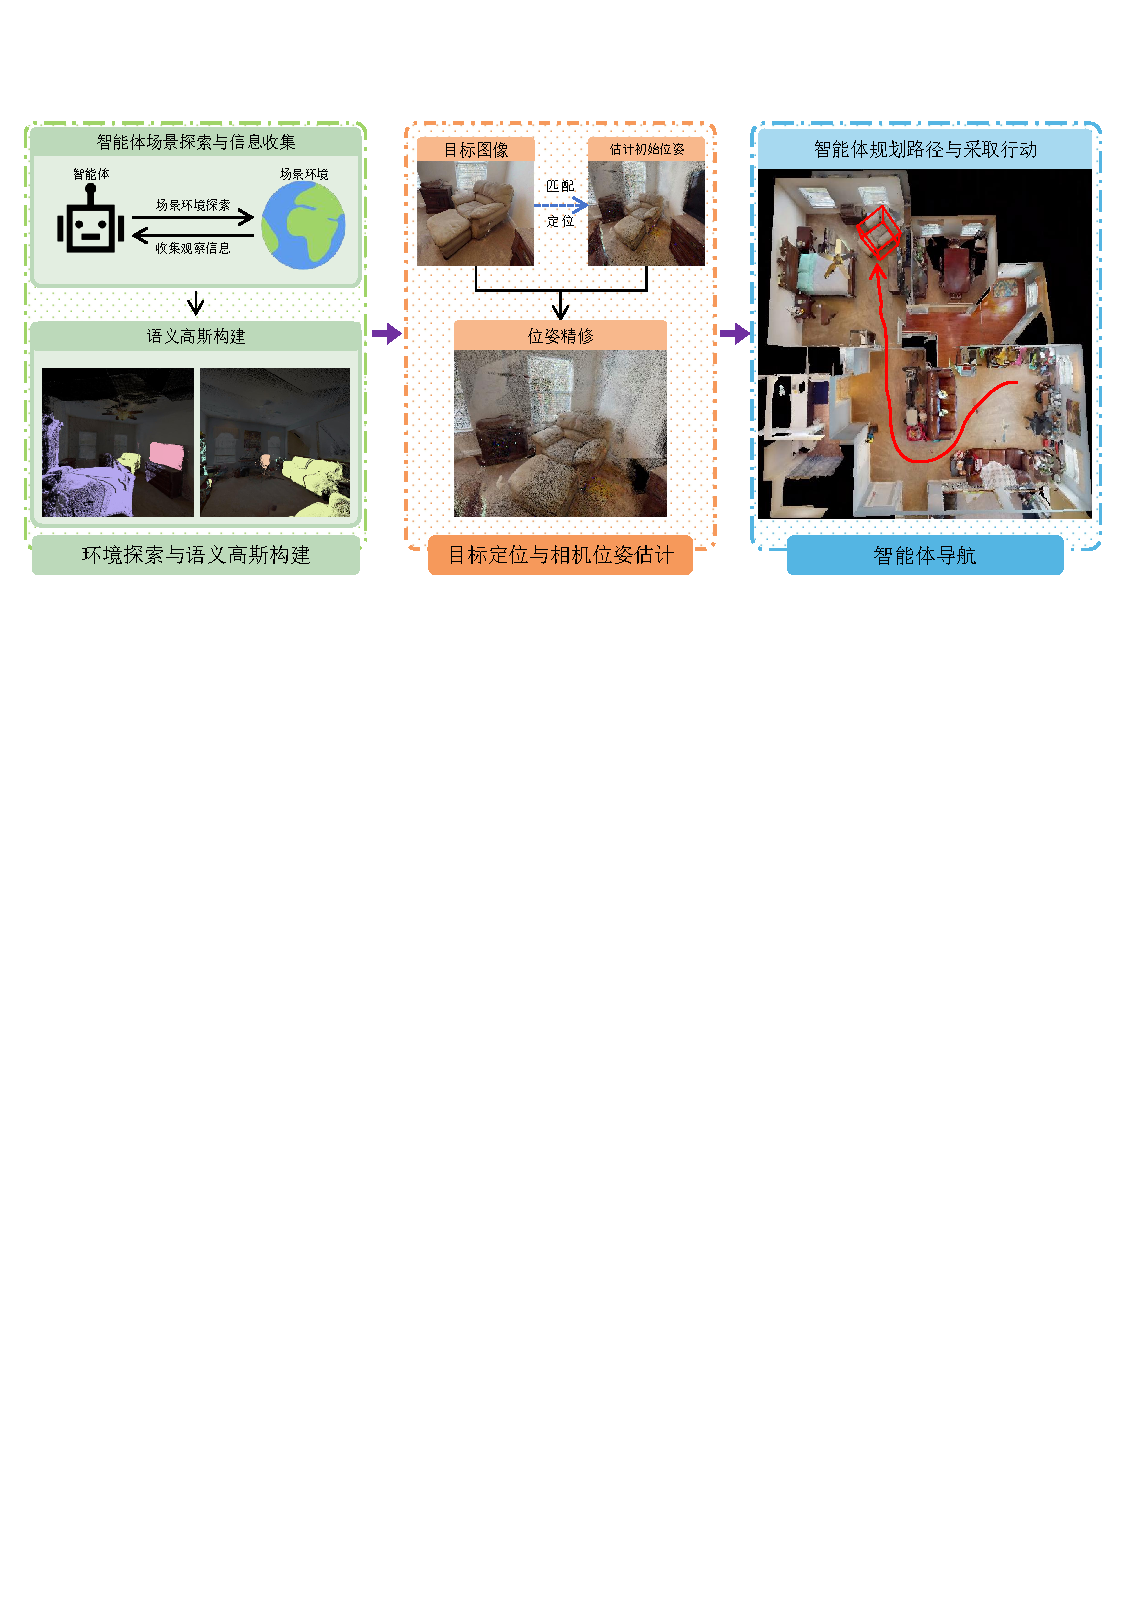
\includegraphics[width=1.0\textwidth]{figures/图标ppt/全流程.pdf}
    \caption{面向视觉导航的模块化框架整体流程}
    \label{fig:任务整体流程}
\end{figure}

在一个全新的环境中，智能体需要先通过探索环境，收集环境观测数据，包括RGB图像、语义、深度等，利用这些信息来构建一个语义高斯地图作为后续的导航基础；
随后，利用已有的构建好的语义高斯地图，与目标图像中的实例物体进行相似度匹配，确定目标物体；
利用包含目标物体的初始训练位姿信息作为初始位姿，通过图像对齐技术逐步从初始位姿对齐到目标图像拍摄位姿，作为最终导航点；
获得最终导航点后，整个IIN任务简化为点导航任务，进而进入智能体动作规划与执行阶段。

下面对这三个主要阶段的核心进行详细描述，GSGuide算法的整体流程如算法\ref{alg:gsguide}所示。
\begin{algorithm}[h!]
    \small
    \SetAlgoLined
    \KwIn{目标图像 $I_g$，初始位姿 $P_0$}
    \KwOut{导航动作序列 $\{a_1, a_2, \ldots, a_T\}$}
    \BlankLine
    \tcc{第一阶段：环境探索与语义高斯地图构建}
    \For{每个探索时间步 $t$}{
        获取观测: $I_t$, $D_t$, $P_t$; 语义分割 $I_t \rightarrow C_t$\;
        高斯致密化: 渲染 $\hat{D}_t$, $\hat{S}_t$, 计算 $M(p)$, 初始化新高斯\;
        \For{每个优化迭代}{
            可微渲染 $\hat{I}_t$, $\hat{D}_t$, $\hat{P}_{seg}$\;
            $\mathcal{L}_{total} = \lambda_{rgb}\mathcal{L}_{rgb} + \lambda_{depth}\mathcal{L}_{depth} + \lambda_{seg}\mathcal{L}_{seg}$\;
            梯度下降更新 $\Psi_i = \{\boldsymbol{c}_i, \boldsymbol{\mu}_i, r_i, o_i, \boldsymbol{l}_i\}$
        }
    }
    \BlankLine
    \tcc{第二阶段：目标定位与相机位姿估计}
    分类 $I_g \rightarrow \hat{\boldsymbol{l}}_g$; 查询地图 $\rightarrow$ 候选集 $\mathcal{O}$\;
    \For{每个 $o_i \in \mathcal{O}$}{
        提取 $\mathcal{P}_i$, 生成视角图像集 $\mathcal{S}_i$
    }
    匹配 $I_g$ 与 $\bigcup_i \mathcal{S}_i \rightarrow \hat{P}_g$\;
    图像对齐精修 $\hat{P}_g \rightarrow P^*$\;
    \BlankLine
    \tcc{第三阶段：智能体导航}
    高斯 $\rightarrow$ 3D体素 $\rightarrow$ 2D BEV $M_{2D}$\;
    FMM计算距离场 $D_{fmm}$\;
    \While{未到达目标}{
        选 $D_{fmm}$ 局部极小点为航点 $w$\;
        根据角度与距离计算并执行动作 $a_t$
    }
    \caption{GSGuide: 基于语义增强3DGS的视觉导航算法}
    \label{alg:gsguide}
\end{algorithm}

\section{环境探索与语义高斯构建}
\subsection{简化后的3D高斯表示}
与原始的3DGS\cite{3DGS}不同，本文所使用的高斯是经过简化的。
遵从原始GaussNav论文，本文保留了原始3D高斯的基元表示核心与可微分渲染能力，将高斯核心参数表示为：
\begin{equation}
    \Psi_i=\{\boldsymbol{c}_i,\boldsymbol{\mu}_i,r_i,o_i,\boldsymbol{l}_i \}
\end{equation}

其中，$i$代表第$i$个语义高斯;
$\boldsymbol{c}_i\in$代表每个高斯的RGB颜色向量；
$\boldsymbol{\mu}_i\in \mathbb{R} ^{3}$表示每个高斯中心坐标；
$r_i\in \mathbb{R}$表示每个高斯的半径；
$o_i\in [0,1]$表示每个高斯的透明度；
$\boldsymbol{l}_i\in \Delta  ^{6}$表示每个高斯所代表的7个语义类别的概率分布，满足非负性与归一化约束。

原始3DGS为了实现照片级别的真实感渲染，使用3阶球谐函数（SphericalHarmonics，SH）编码每个高斯的颜色。
每个高斯的RGB通道各需要9个颜色系数总共27个颜色系数。
这样可以实现同一个物体的不同观察视角对应的不同颜色编码，以达到例如金属物体不同角度的反光颜色不一样的效果。

而IIN任务中，导航的核心需求是识别物体、理解几何场景，对实时性要求较高，而不是照片级别的真实感渲染。
因此本文抛弃了基于球谐函数的颜色编码方式，而是将每个高斯简化为只使用3维RGB颜色向量的颜色编码方式。
具体原因如下：
\begin{enumerate}
    \item 物体的整体颜色和纹理特征已经足够支撑实例级匹配需求；
    \item Habitat-Sim模拟器提供的虚拟场景中本身并没有基于球谐函数的不同角度的颜色表示方式。
\end{enumerate}
这样以来，渲染质量虽略有下降，但换来的是参数量减少90\%，渲染速度大幅提升，更加贴合IIN任务的实时性需求。

同时，本文还将高斯约束为各向同性（仅保留单个缩放因子）。原始3DGS使用各向异性来拟合三维场景结构。
对于每个高斯而言，各个方向因缩放因子不同，不同的高斯看起来更像是大小、朝向均不同的椭球体。
这需要每个高斯存储3个缩放因子，分别对应$x$，$y$，$z$三个轴的长度以及1个四元旋转参数来表示椭球体的方向。
这种方法对于拟合平面、柱体等平面或者细长结构的拟合能力很强，几何重建度较高。

而本文则进一步将所有高斯约束为各向同性，退化为一个完美球体。
这样以来，三个轴的缩放因子完全相同，只需要一个标量半径$r$即可表示；球形的各向同性使得高斯不再旋转参数。
这原因如下：
\begin{enumerate}
    \item 智能体在探索与导航时只需知道障碍物与物体的大致位置，不需要毫米级别的精确度；
    \item 球形高斯已足够表示场景的整体结构与物体的实例形状；
\end{enumerate}
这种方法进一步降低了参数数量，从原始的3个缩放因子与一个旋转四元数变为进一个标量半径$r$，几何参数减少86\%，在进一步降低内存占用的同时显著的提升了渲染效率，贴合IIN任务的实时性要求。

\subsection{语义高斯构建}
原始的3DGS的RGB渲染过程如下：给定一组3D高斯和相机位姿，首先将所有高斯按照深度从近到远进行排序；
随后将每个3D高斯投影到图像平面形成2D椭圆；
最后通过alpha混合操作按照深度顺序累加每个像素的颜色贡献，得到最终的渲染图像。
像素$p=(u,v)$的渲染颜色可以表示为：
\begin{equation}
    \hat{I}(p)=\sum_{i=1}^{n}\boldsymbol{c}_i f_i(p)\prod _{j=1}^{i-1}(1-f_j(p))
\end{equation}
% 在详细解释一下参数
其中，权重函数$f_i(p)$定义为：
\begin{equation}
    f_{i}(\boldsymbol{x})=o \exp{(- \frac{\Vert \boldsymbol{x}-\boldsymbol{\mu} \Vert ^{2}}{2r^2})}
\end{equation}
其中，通过3D高斯的投影计算得到2D高斯的中心$\boldsymbol{\mu} $和半径$r$：
\begin{equation}
    \boldsymbol{\mu} ^{2D}=K \frac{E_t\boldsymbol{\mu} }{d}, r^{2D}=\frac{fr}{d}, d=(E_t\boldsymbol{\mu} )_z
\end{equation}
公式中，$K$为相机内参矩阵，$E_t$为包含了相机旋转和平移信息的外参矩阵，$f$为相机的焦距，$d$为第$i$个高斯在相机坐标系下的深度值。

% 语义高斯是一个迭代的过程，包含两个交替执行的步骤：高斯致密化与语义地图更新。
% 如图\ref{fig:R-c}所示，
% \begin{figure}[htbp]
%     \centering
%     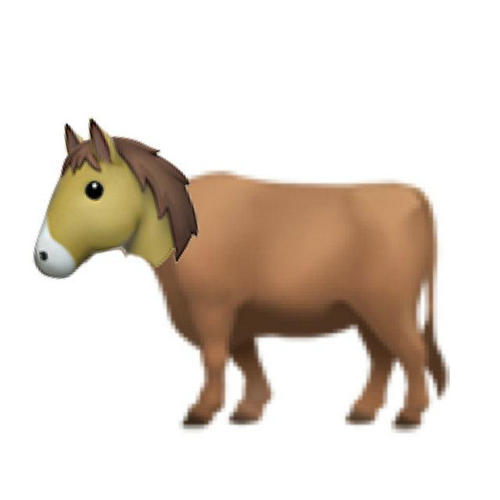
\includegraphics[width=0.8\textwidth]{figures/R-C.jpg}
%     \caption{语视觉导航的模块化框架整体流程图}
% \end{figure}
% 高斯致密化是指在每一帧新观测到来时初始化新的高斯，而语义高斯更新步骤则是通过可微渲染技术优化所有高斯参数。

与原版3DGS不同，本文提出的GSGuide框架可同时可微渲染深度图和轮廓图，用于后续的高斯致密化和参数更新。
像素$p$处的渲染深度$\hat{D}(p)$和轮廓$\hat{S}(p)$分别为：
\begin{equation}
    \hat{D}(p)=\sum_{i=1}^{n}d_i f_i(p)\prod _{j=1}^{i-1}(1-f_j(p))
\end{equation}

\begin{equation}
    \hat{S}(p)=\sum_{i=1}^{n}r_i f_i(p)\prod _{j=1}^{i-1}(1-f_j(p))
\end{equation}


语义高斯的迭代渲染过程包含两个交替执行的步骤：高斯致密化与语义地图更新。
高斯致密化是指在每一帧新观测到来时初始化新的高斯，而语义高斯更新步骤则是通过可微渲染技术优化所有高斯参数。
流程如图\ref{fig:语音渲染流程}所示，
\begin{figure}[htbp]
    \centering
    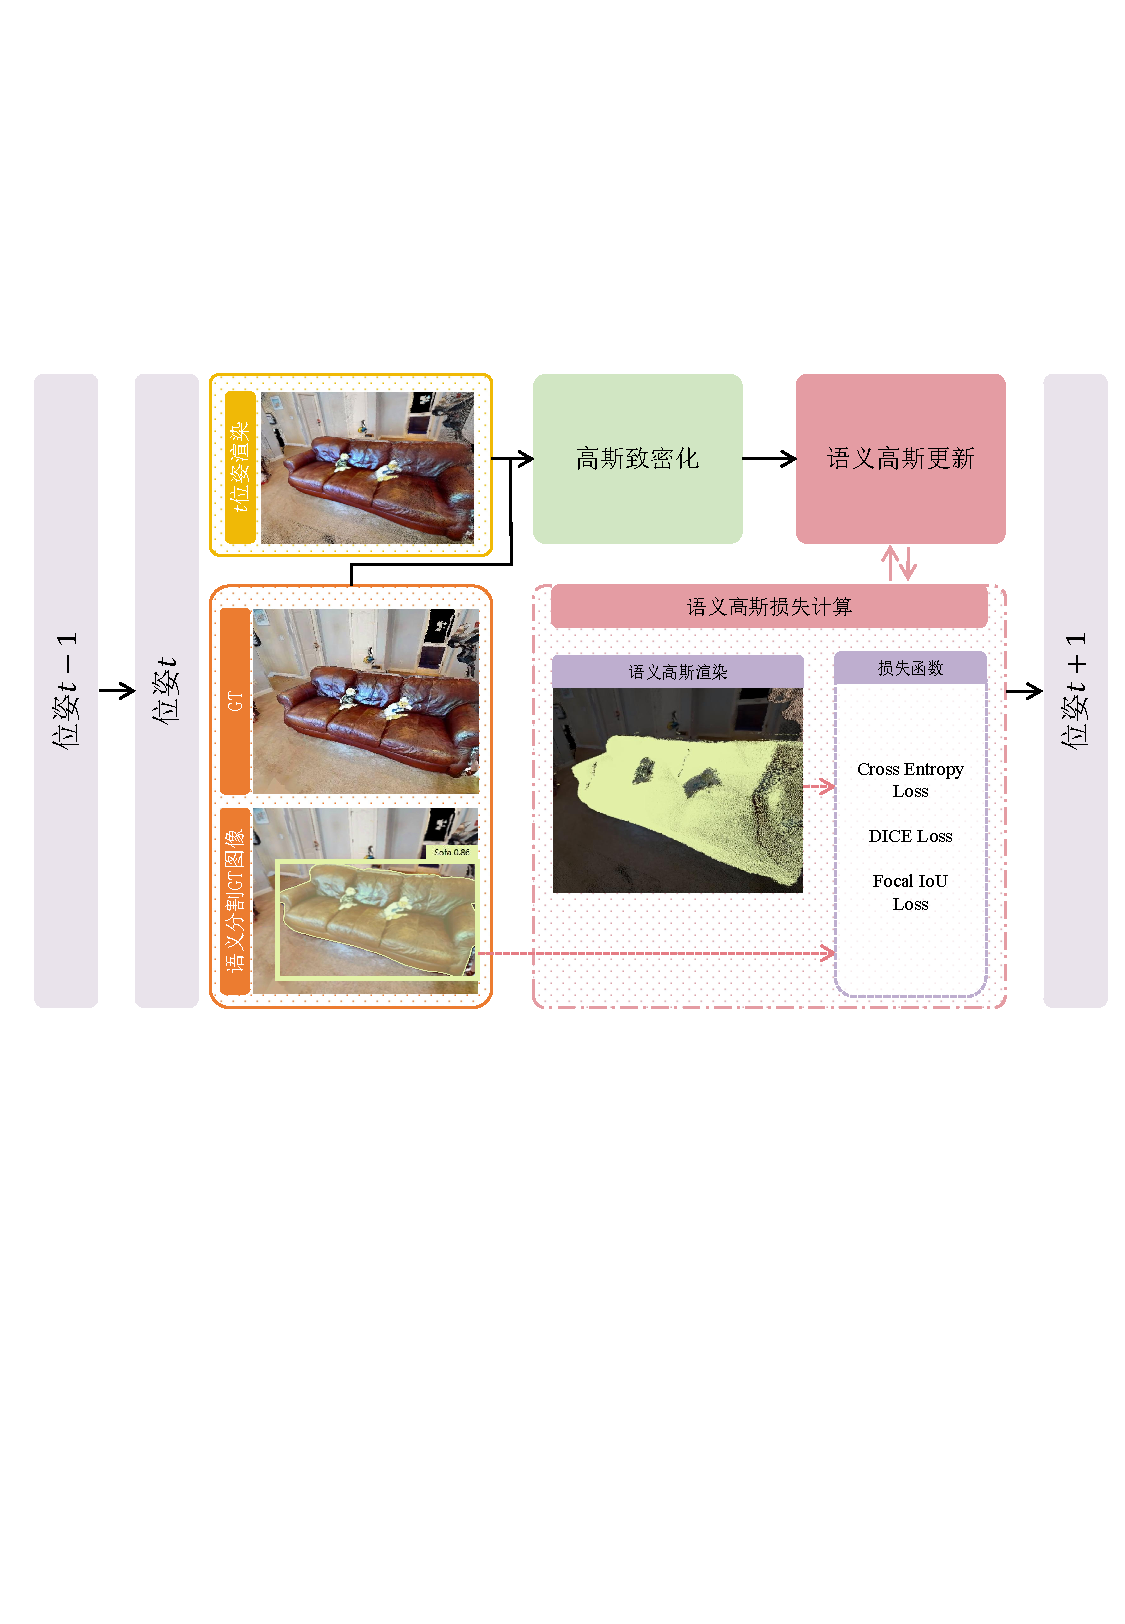
\includegraphics[width=1.0\textwidth]{figures/图标ppt/语义更新过程.pdf}
    \caption{语义高斯渲染流程}
    \label{fig:语音渲染流程}
\end{figure}
智能体的RGB观测通过Yolo26模型进行语义分割，得到分割结果$C_t$。
在高斯致密化过程中的高斯初始化阶段，为每个高斯的语义标签$l$赋予初始值。
随后，通过可微渲染技术，将所有高斯的语义渲染结果与真实语义图进行对比，计算出所有高斯的语义损失，进行参数更新。

GaussNav在实现过程中仅将语义信息赋予高斯离散语义标签，在优化阶段跳过了梯度跟踪。
本文通过优化语义标签渲染过程，采用与RGB相同的渲染逻辑，但不参与$\alpha$混合操作，而是选取贡献度最大的高斯所带有的语义为每个像素渲染一个$v$维语义向量，经$softmax$将$v$维向量表示为各语义类别概率，实现了语义标签的梯度跟踪，实现后续的语义监督与优化过程。

在时刻$t$，高斯致密化会通过比较基于$t-1$时刻高斯在当前位姿$P_t$的渲染结果与真实RGB观测图像，在现有已经构建好的高斯因没有覆盖而无法表示的区域新增高斯。
本文参考Keetha\cite{keetha2024splatam}等人方法，基于致密化掩码$M(p)$确定需要添加高斯的像素位置。
计算公式如下：
\begin{equation}
    M(p)=(\hat{S}(p)<0.5)+(D(p)<\hat{D}(p))(L_1(\hat{D}(p))>50 \cdot MDE)
\end{equation}
式中，$(\hat{S}(p)<0.5)$表示现有高斯密度不足的区域，$(D(p)<\hat{D}(p))(L_1(\hat{D}(p))>50 \cdot MDE)$表示真实深度中位于预测深度方向的前方且深度误差大于50倍中值深度误差（MDE）的区域。

完成当前帧的高斯致密化后，本文通过可微渲染和 梯度下降优化更新所有高斯中的所有参数。
这一过程等价于键辐射场拟合到已知位姿图像的经典问题，通过计算RGB、深度、语义分割损失以及他们的加权损失，来更新每个高斯中的参数。
具体而言，总损失定义如下：
\begin{equation}
    \mathcal{L} _{total}=\lambda _{rgb} \mathcal{L}_{rgb}+\lambda _{depth} \mathcal{L}_{depth}+\lambda _{seg} \mathcal{L}_{seg}
\end{equation}

其中，$\mathcal{L} _{rgb}$为渲染图像与真实RGB观测图像的$L_1$和SSIM组合损失，具体定义为：
\begin{equation}
    \mathcal{L}_{rgb}=\lambda_{L1} \cdot L1(I_{render},I_{gt})+\lambda_{SSIM}\cdot (1-SSIM(I_{render},I_{gt})) 
\end{equation}
深度损失定义为：
\begin{equation}
    \mathcal{L}_{depth}=\mathcal{L} _{depth}=\frac{1}{| M | }\Sigma _{(h,w)\in M}|D_{render}[h,w]-D_{gt}[h,w]|
\end{equation}
其中，$D_{render} \in \mathbb{R} ^{1\times H \times W}$代表渲染得到的深度图，$D_{gt} \in \mathbb{R} ^{1\times H \times W}$代表真实深度图，$M$代表有效像素掩码，$|M|$代表掩码$M$中有效像素的数量。

语义损失包含了$\mathcal{L} _{ce}$交叉熵损失、$\mathcal{L} _{dice}$DICE损失，以及基于IoU的Focal IoU损失$\mathcal{L} _{focal\_iou}$。
语义总损失定义为：
\begin{equation}
    \mathcal{L}_{seg}=\lambda_{ce} \mathcal{L}_{ce}+\lambda_{dice} \mathcal{L}_{dice}+\lambda_{focal\_iou} \mathcal{L}_{focal\_iou}
\end{equation}

交叉熵损失是图像分割和目标分类中最基础的损失函数。其核心思想是对于每个像素预测出一个概率分布，交叉熵衡量这个预测分布与真实标签分布之间的相似程度。
真实标签对应类别的预测概率越接近$1$，损失就越小，反之则越大。
交叉熵损失定义为：
\begin{equation}
    \mathcal{L} _{ce}=CrossEntropy(P_{seg},Y_{gt})
\end{equation}
其中，$P_{seg} \in \mathbb{R} ^{1\times C \times H \times W},Y_{gt}\in\mathbb{N} ^{1\times 1\times H\times W}$,$P_{seg}$表示语义渲染概率图，$Y_{gt}$表示真实语义标签，$C$表示渲染通道数，即语义类别数。

Dice 损失函数源于 Sørensen-Dice 系数，是图像分割任务中广泛采用的一致性评价指标，其值越接近 1 表示预测区域与真实标注区域的重叠程度越高。Dice 损失定义为 $1$ 减去 Dice 系数，因此优化 Dice 损失本质上是对评价指标本身的直接优化，这一特性使其在动机层面相较于交叉熵损失更契合分割任务的核心目标。特别在小目标分割和类别不平衡场景下，Dice 损失能够更有效地引导模型关注边界细节和小区域的精确分割。

Dice损失定义为：
\begin{equation}
\begin{aligned}
\text{Intersection}_c &= \sum_{h=1}^H\sum_{w=1}^W \mathbf{P}_{\text{semantic}}[0,c,h,w] \cdot \mathbf{Y}_{\text{gt\_onehot}}[0,c,h,w], \\
\text{Union}_c &= \sum_{h=1}^H\sum_{w=1}^W \mathbf{P}_{\text{semantic}}[0,c,h,w] + \sum_{h=1}^H\sum_{w=1}^W \mathbf{Y}_{\text{gt\_onehot}}[0,c,h,w], \\
\text{Dice}_c &= \frac{2 \cdot \text{Intersection}_c + \epsilon}{\text{Union}_c + \epsilon}, \\
\mathcal{L}_{\text{dice}} &= 1 - \frac{1}{C} \sum_{c=1}^C \text{Dice}_c,
\end{aligned}
\end{equation}

其中各参数定义如下：
\begin{itemize}
    \item $\mathbf{P}_{\text{semantic}} \in \mathbb{R}^{1 \times C \times H \times W}$：模型预测的语义概率图，第$[0,c,h,w]$个元素表示位置$(h,w)$处属于类别$c$的概率，取值范围为$[0,1]$；
    \item $\mathbf{Y}_{\text{gt\_onehot}} \in \mathbb{R}^{1 \times C \times H \times W}$：真实语义标签的one-hot编码，当位置$(h,w)$的真实类别为$c$时，$\mathbf{Y}_{\text{gt\_onehot}}[0,c,h,w] = 1$，否则为0；
    \item $\text{Intersection}_c$：第$c$类的预测结果与真实标签的逐元素乘积之和，即两类区域的交集像素数；
    \item $\text{Union}_c$：第$c$类的预测概率图与真实标签的逐元素求和，即两类区域的并集像素数（未扣除重叠部分）；
    \item $\text{Dice}_c$：第$c$类的Dice系数，取值范围为$[0,1]$，值越大表示预测与真实的一致性越高；
    \item $C$：语义类别总数；$H, W$：特征图的高度和宽度；
    \item $\epsilon = 1e-5$：数值稳定性平滑项，避免计算时分母为零导致数值不稳定。
\end{itemize}


Focal 损失函数由 Lin\cite{focal} 等人提出，旨在解决密集目标检测与分割任务中难易样本极端不均衡的问题。
在3D高斯语义渲染任务中，不同语义类别（如背景与前景、小物体与大物体）的像素数量存在显著差异，传统IoU损失对简单样本和困难样本同等对待，导致模型训练偏向于占主导地位的类别。为此，本文引入Focal IoU损失，通过动态加权机制聚焦于难分类样本，定义为：
\begin{equation}
\begin{aligned}
\text{Intersection}_c &= \sum_{h=1}^H\sum_{w=1}^W \mathbf{P}_{\text{semantic}}[0,c,h,w] \cdot \mathbf{Y}_{\text{gt\_onehot}}[0,c,h,w], \\
\text{Union}_c &= \sum_{h=1}^H\sum_{w=1}^W \mathbf{P}_{\text{semantic}}[0,c,h,w] + \sum_{h=1}^H\sum_{w=1}^W \mathbf{Y}_{\text{gt\_onehot}}[0,c,h,w] - \text{Intersection}_c, \\
\text{IoU}_c &= \frac{\text{Intersection}_c + \epsilon}{\text{Union}_c + \epsilon}, \\
\text{FocalIoU}_c &= 1 - \text{IoU}_c \cdot \left(1 - (1 - \text{IoU}_c)^\gamma\right), \\
\mathcal{L}_{\text{focal\_iou}} &= \frac{1}{C} \sum_{c=1}^C \text{FocalIoU}_c,
\end{aligned}
\end{equation}

其中各参数定义如下：
\begin{itemize}
    \item $\mathbf{P}_{\text{semantic}} \in \mathbb{R}^{1 \times C \times H \times W}$：模型预测的语义概率图，第$[0,c,h,w]$个元素表示位置$(h,w)$处属于类别$c$的概率；
    \item $\mathbf{Y}_{\text{gt\_onehot}} \in \mathbb{R}^{1 \times C \times H \times W}$：真实语义标签的one-hot编码，当位置$(h,w)$的真实类别为$c$时，$\mathbf{Y}_{\text{gt\_onehot}}[0,c,h,w] = 1$，否则为0；
    \item $\text{Intersection}_c$：第$c$类的预测结果与真实标签的交集像素数；
    \item $\text{Union}_c$：第$c$类的预测结果与真实标签的并集像素数；
    \item $\text{IoU}_c$：第$c$类的交并比，衡量预测区域与真实区域的重合程度；
    \item $\gamma = 2.0$：Focal参数，控制难分类样本的权重增强程度，$\gamma$越大，困难样本获得的权重越高；
    \item $\epsilon = 1e-5$：数值稳定性平滑项，避免计算IoU时分母为零；
    \item $C$：语义类别总数；$H, W$：特征图的高度和宽度。
\end{itemize}

Focal IoU损失通过在标准IoU损失\cite{yu2016unitbox}基础上引入调制因子$(1 - \text{IoU}_c)^\gamma$实现动态样本加权：当$\text{IoU}_c$接近1（简单样本）时，调制因子趋近于0，损失被显著降低；当$\text{IoU}_c$较小（困难样本）时，调制因子趋近于1，损失保持较大值。这种机制迫使模型在训练过程中更多地关注语义边界模糊、类别混淆等困难样本，从而提升整体语义渲染的准确性和鲁棒性。


联合使用三个不同的语义损失从像素级、区域级和困难样本三个维度对分割结果施加互补约束。
交叉熵损失提供逐像素的分类监督，确保每个像素点的预测概率分布与真实标签一致；
Dice损失从集合重叠的角度优化整体一致性，特别关注小目标和前景区域的精确分割；
Focal IoU损失则动态调整难易样本的权重，迫使模型聚焦于语义边界模糊、类别混淆等困难样本。
三者协同作用形成多层次、多粒度的语义监督体系：交叉熵损失保证基础分类准确性，Dice损失增强区域一致性，Focal IoU损失提升困难样本的识别能力，从而显著提升语义高斯地图的渲染质量，为后续的目标定位与导航任务奠定坚实基础。
% 消融实验结果（如表\ref{tab:ablation_semantic}所示）验证了该多损失联合策略的有效性，完整三损失组合在所有语义渲染指标上均取得了最优性能。

\section{目标定位与相机位姿估计}
利用构建完成的语义高斯地图，本文提出高斯导航算法，流程如图\ref{fig:导航流程图}所示。
\begin{figure}[htbp]
    \centering
    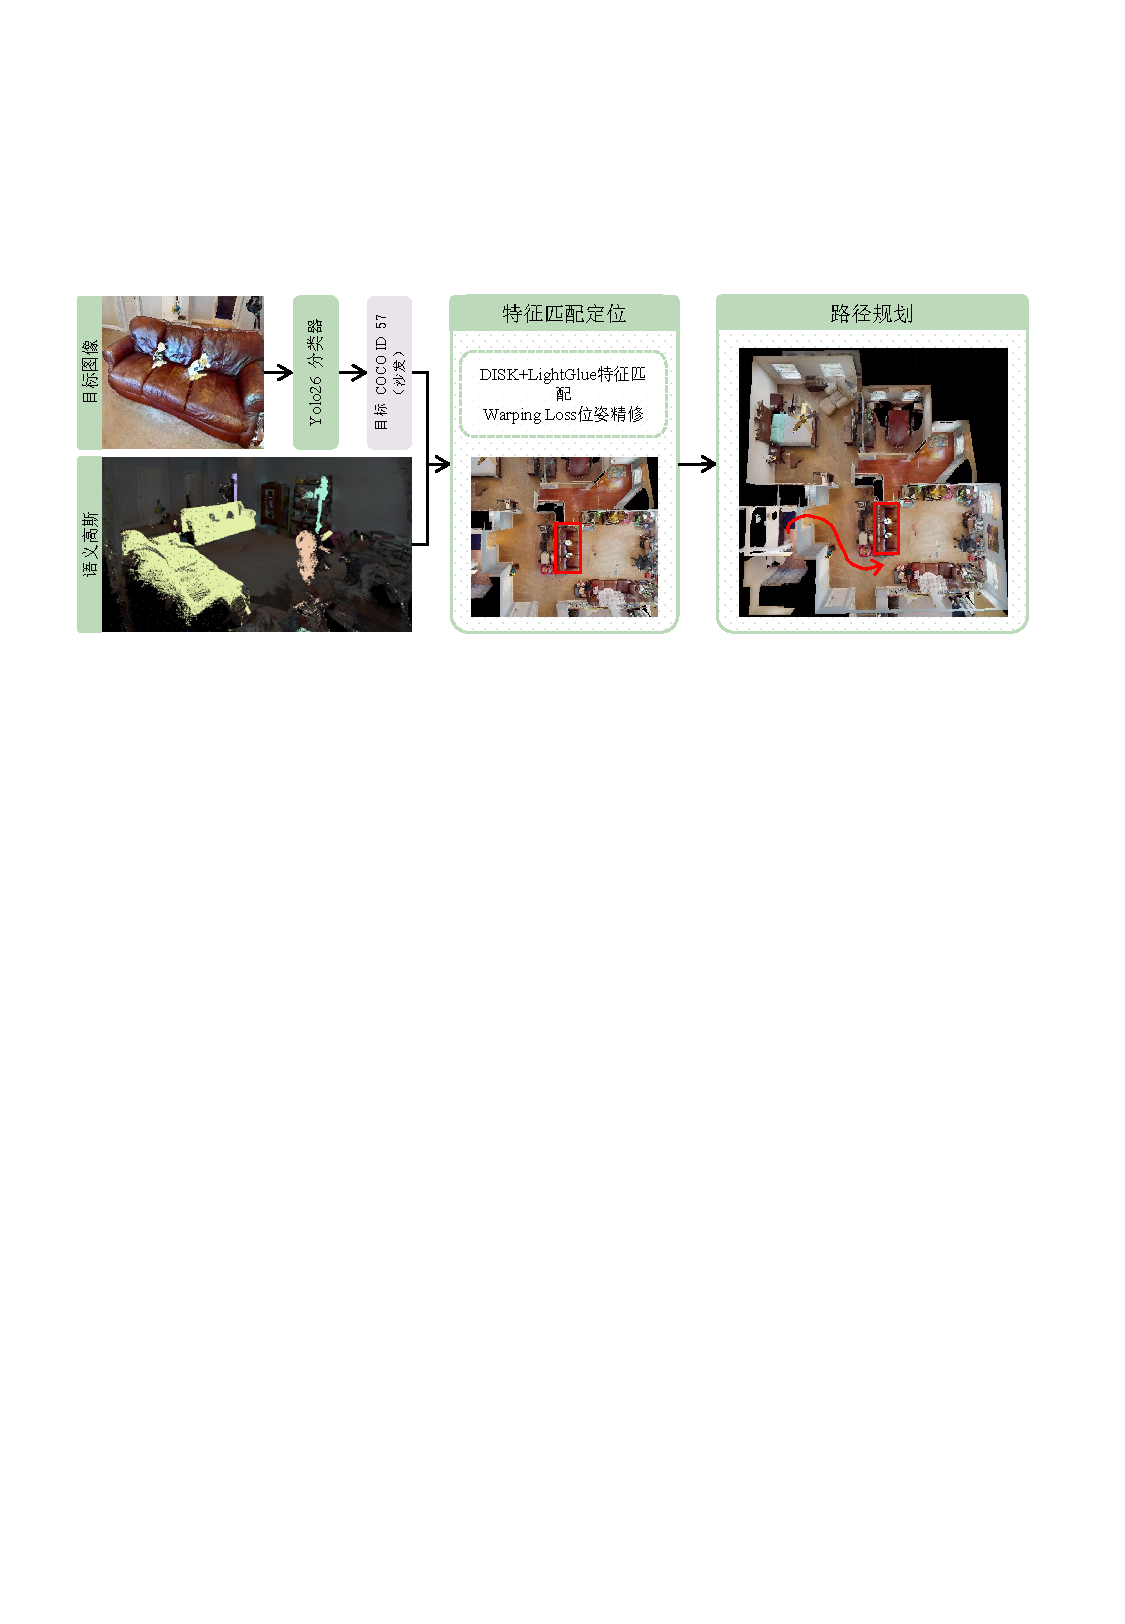
\includegraphics[width=1.0\textwidth]{figures/图标ppt/导航流程图.pdf}
    \caption{目标定位与路径规划流程}
    \label{fig:导航流程图}
\end{figure}

首先，对目标图像$I_g$进行分类，预测目标物体的语义标签$\boldsymbol{\hat{l}}_{g}$；
然后利用该语义标签查询语义高斯地图中所有同类别实例物体，并与目标图像进行匹配，从而确定初始位姿$\hat{P}_{g}$；
最后通过路径规划模块生成可行路径并输出智能体动作序列。

\subsection{分类器}
考虑到直接将目标图像与场景中所有可导航点的渲染结果进行匹配会导致搜索空间过于庞大，导致计算效率极低。
因此，本文首先通过分类器预测目标图像中的物体实例语义类别；
得到类别后信息后，可以在场景中通过检索相同类比的物体进行后续匹配，进而大幅度降低搜索空间，提升效率。

本文使用Yolo团队官方提供的预训练好的Yolo26\cite{Yolo26}模型作为分类器进行分类。

\subsection{匹配与定位}
根据分类器预测的目标类别$\hat{l}_g$，提取语义高斯地图中包含所有该类别的候选物体实例，加载相应的拍摄相机位姿。

假设相机坐标系到Habitat世界坐标系的转换矩阵为$c2w$，候选物体在该相机视角坐标系下的平移向量为$\boldsymbol{t}_c^{o}$。
本文定义物体到世界坐标系的旋转矩阵由前向、右向和向上三个向量构成：
前向向量为从训练视角相机指向候选物体的向量$\boldsymbol{t}_c^{o}$，向上的向量定义为[0,-1,0]，右向向量与前向和向上的向量共同构成右手坐标系。
则物体到世界坐标系的平移向量$\boldsymbol{t}_w^{o}$为：
\begin{equation}
    \boldsymbol{t}_w^{o}={c2w} \times \boldsymbol{t}_c^{o}
\end{equation}

旋转矩阵与平移向量共同构成物体到世界坐标系的刚体变换矩阵$o2w$。

本文定义围绕y轴和x轴的旋转矩阵分别为$\boldsymbol{R}_{y}(\theta)$，$\boldsymbol{R}_{x}(\theta)$，用于后续生成水平和垂直方向上的新视角。
水平和垂直方向新视角生成方式如下：
\begin{equation}
    c2w_{h}(\theta)=o2w\times \boldsymbol{R}_{y}(\theta)\times w2o\times c2w
\end{equation}
\begin{equation}
    c2w_{v}(\theta)=o2w\times \boldsymbol{R}_{x}(\theta)\times w2o\times c2w
\end{equation}

设每个候选实例$i$所对应的候选图像集合为$S_{i}$。
当场景中拥有$n$个与目标同类别候选实例时，所有候选的渲染图像集合为：
\begin{equation}
    S={S_1,S_2,...,S_n} \quad for i=1,2,...,n
\end{equation}

针对候选图像，本文采用LightGlue+DISK\cite{disk,lightglue}进行特征点提取与匹配作为初始估计位姿，再使用GSplatLoc\cite{gsplatloc}提出的Warping Loss图像扭曲技术基于粗位置对齐目标图像拍摄相机位姿。
具体而言，在分类器输出类别信息后，搜索范围可缩小在相同类别的候选实例中，目标物体的识别可形式化为选择匹配点数量最多的候选实例：
\begin{equation}
    i_{max}=argmax\{max_{s\in S_{1}}\Omega (s),max_{s\in S_{2}}\Omega (s),...max_{s\in S_{n}}\Omega (s)\}
\end{equation}

式中$\Omega (\cdot)$表示渲染图像$s$和目标图像$I_g$中提取关键点坐标及其特征描述子：
\begin{equation}
    (K_t,V_t)=DISK(s), \quad (K_g,V_g)=DISK(I_g)
\end{equation}
然后使用LightGlue算法进行特征匹配，得到关键点匹配对：
\begin{equation}
    (\hat{K}_t,\hat{K}_g)=LightGlue((K_t,V_t),(K_g,V_g))
\end{equation}
匹配关键点数量即为$\Omega$的值。
匹配点数量最多的候选实例即为目标物体，选取其位姿作为初始位姿。

确定目标实例后与初始位姿$(\boldsymbol{R},\boldsymbol{t})$后，根据初始位姿$(\boldsymbol{R},\boldsymbol{t})$渲染图像$q_r$以及对应的深度图$d_r$，随后最小化 Warping Loss 来优化最终的位姿$(\boldsymbol{R}^{\prime},\boldsymbol{t}^{\prime})$。

Warpping Loss定义为渲染图像与目标图像的所有像素级别的RGB差异总和：
\begin{equation}
    \mathcal{L}_{rgb-warp}=\Sigma _{p_i} \| Y(q,W(p_i,\boldsymbol{R},\boldsymbol{t}))-Y(q_r,p_i)\| _2
\end{equation}
其中，扭曲函数$W(\cdot)$定位为：
\begin{equation}
    W(p_i,\boldsymbol{R},\boldsymbol{t},\boldsymbol{R}^{\prime},\boldsymbol{t}^{\prime})=\Pi (\boldsymbol{R}(\boldsymbol{R}^{\prime -1}\Pi ^{-1}(p_i,z_r(p_i))-\boldsymbol{R}^{\prime -1}\boldsymbol{t}^{\prime})+\boldsymbol{t})
\end{equation}
其中，$Y(q_r,P_i)\in \mathbb{R} ^{3}$表示渲染图像$q_r$上位于$i$处的像素$p_i\in \mathbb{R} ^{3}$的RGB颜色值。
扭曲函数$W(\cdot)$通过对参考图像$q_r$上的像素$p_i$执行坐标变换，找到其在目标图像$q$上对应的像素。
具体而言，函数$W$利用渲染深度$z_r$将像素$p_i$反投影到渲染图像$q_r$对应的三维相机坐标系中，再通过优化后的位姿$(\boldsymbol{R}^{\prime},\boldsymbol{t}^{\prime})$将其转换到目标图像$q$的相机坐标系，最终投影到目标图像$q$的平面上。

使用迭代优化后的估计位姿$(\boldsymbol{R}^{\prime},\boldsymbol{t}^{\prime})$作为目标物体拍摄的相机位姿，将其转换为世界坐标系下的位置与智能体可导航点。
至此，IIN任务被转化为点目标导航任务。

在这里，本文提供一个实际成功基于初始位姿精修成功的案例。
如图\ref{fig:位姿精修成功案例}所示：
\begin{figure}
    \centering
    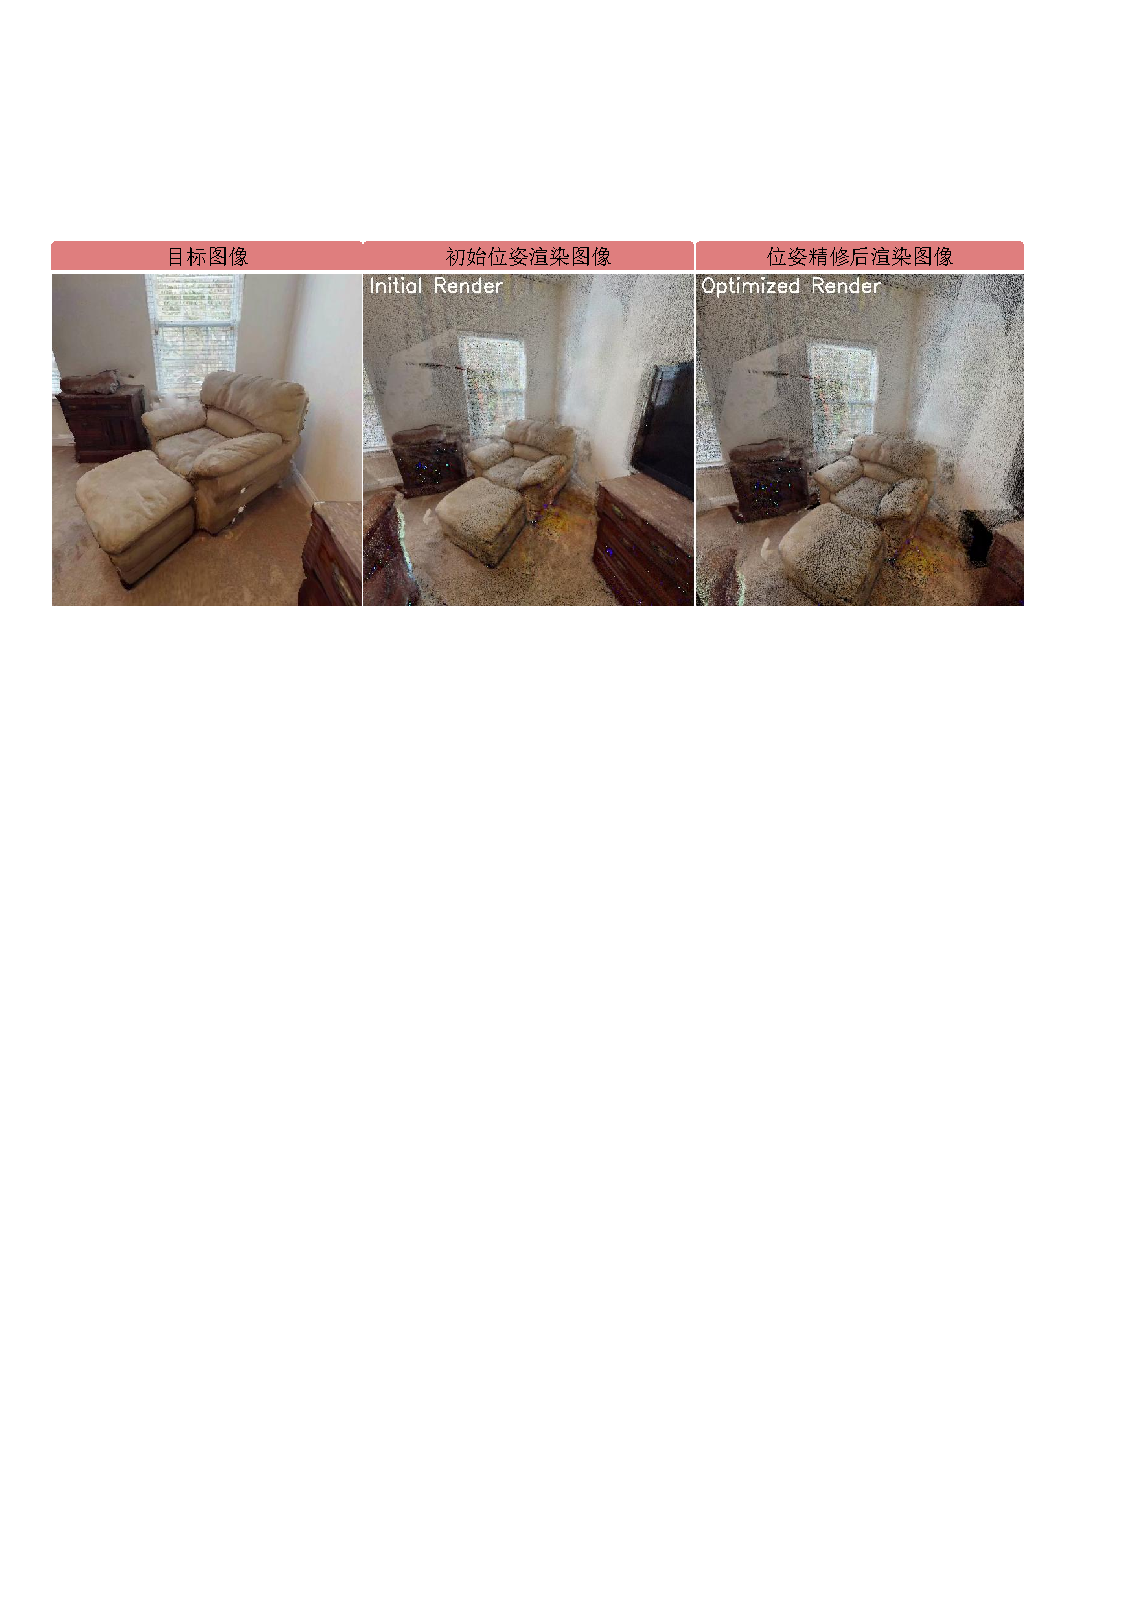
\includegraphics[width=1.0\textwidth]{figures/成功进行位姿精修图片.pdf}
    \caption{位姿精修成功案例可视化}
    \label{fig:位姿精修成功案例}
\end{figure}
左边为智能体接收到的目标图像，中间为初始粗位姿下的渲染图像，右侧为经过Warping Loss后的渲染图像。
可以看出精修后拍摄位姿更加贴近于目标图像的拍摄位姿。


\section{智能体导航} 
% 语义高斯地图并非专为路径规划设计，因此本文首先将其转换为点云（每个高斯对应点云中的一个点），然后将点云体素化为 3D 体素网格M3D​，最后将 3D 体素网格投影为 2D 鸟瞰图（BEV）网格M2D。
语义高斯梯度并非为路径规划设计，因此本文首先基于优化后位姿观察得到的高斯转换为点云，然后将点云体素化为3D体素网格M3D，最后将3D体素网格投影为2D鸟瞰图（BEV）网格M2D。
本文使用语义高斯的 2D 投影而非预探索阶段的 2D 几何地图，以保持整个流程表示的一致性。
由于语义高斯使用深度图像生成的点云进行初始化，且在优化过程中不进行高斯剪枝，因此其 2D 投影与预探索阶段的 2D 几何地图本质上是等价的。
给定 2D BEV 网格地图M2D智能体起始位置和目标位置，本文使用快速行进法（FMM）生成最短距离场。
距离场中的每个点存储从起始点到该点的最短路径长度。
智能体在其运动范围内选择距离场的局部极小值点作为下一个航点，确保路径不与障碍物相交。
根据当前状态与航点的角度和距离，智能体计算并执行相应动作。
迭代上述过程直至到达目标位置

在这里，本文提供一个实际导航成功案例的可视化过程图。
如图\ref{fig:导航移动示例图片}所示，
\begin{figure}[htbp]
    \centering
    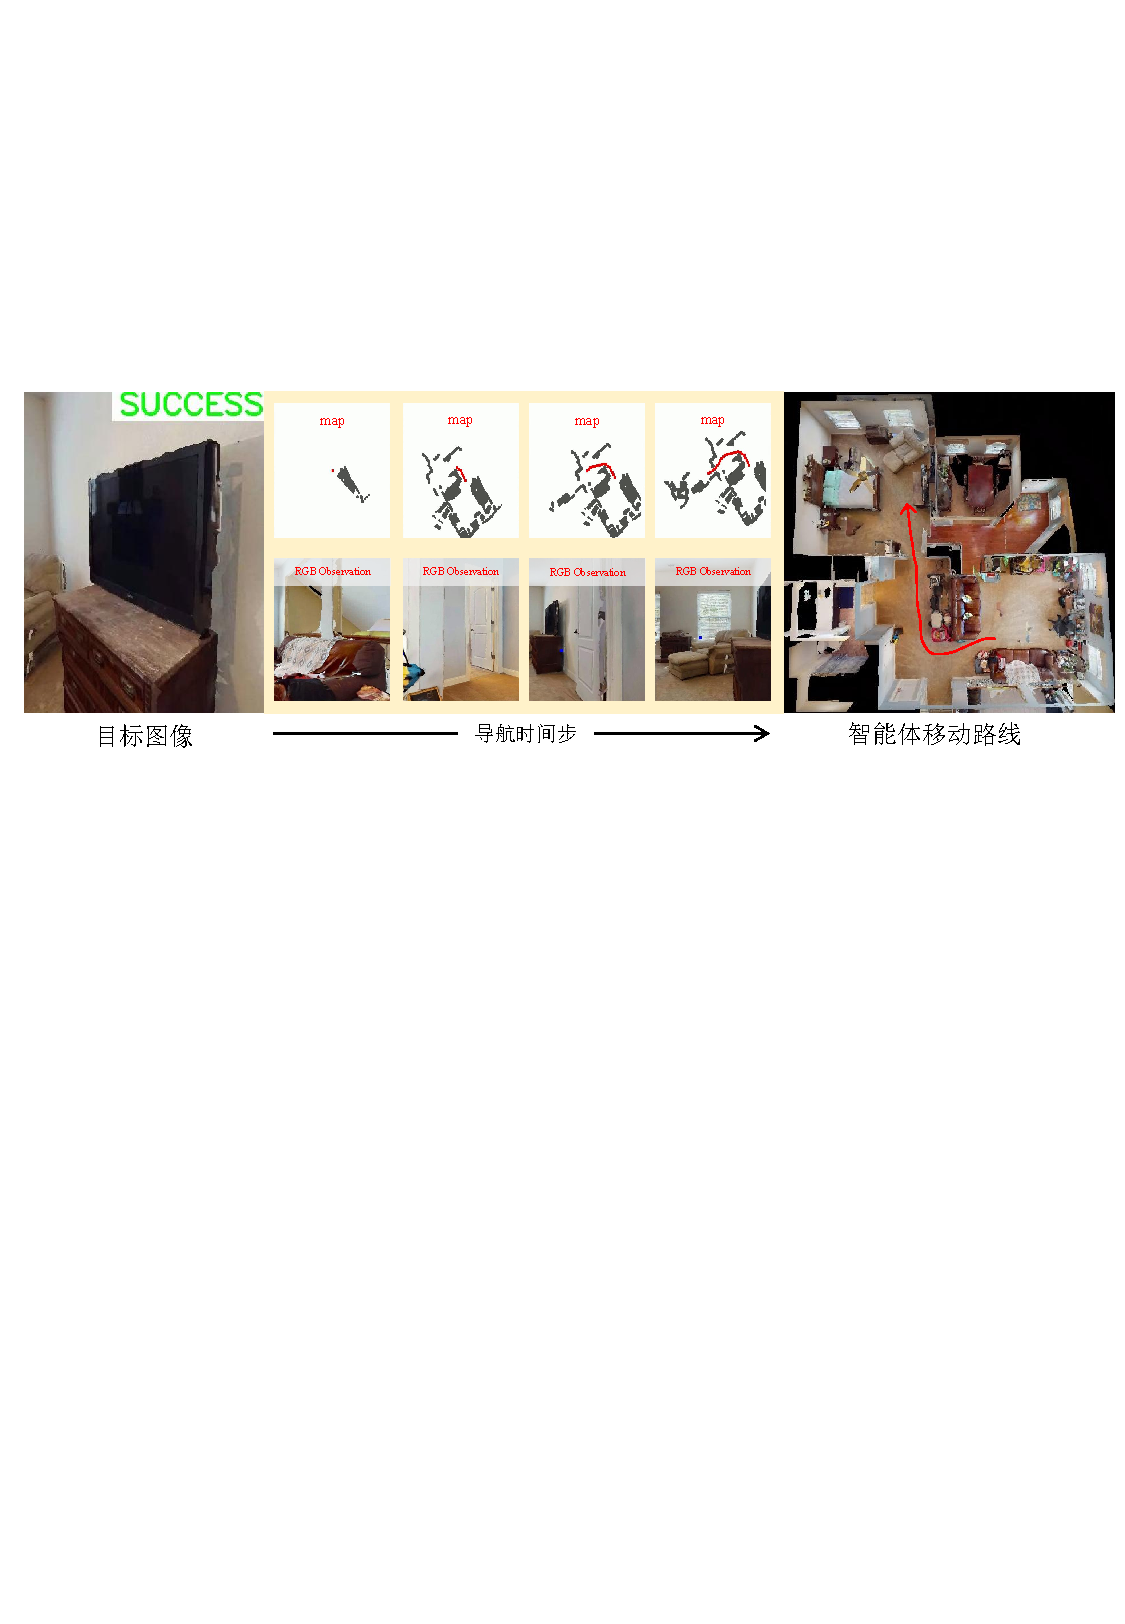
\includegraphics[width=1.0\textwidth]{figures/图标ppt/导航成功案例.pdf}
    \caption{导航成功案例可视化过程}
    \label{fig:导航移动示例图片}
\end{figure}
当智能体在环境中被随机初始化时，系统会向其提供一张展示目标物体的目标图像。
智能体利用已构建好的高斯以及处理过目标位置，并向目标物体移动，最终到达目标物体。

% 写一下语义高斯渲染的公式，完善语义渲染逻辑表示
% 写一下实际应用中的相机参数设置，焦距设置
% 在线3D高斯重建
% 高斯贡献度的问题
%warpingloss学习率调整器件
